% textidote: ignore begin
\section{System Choice}\label{sec:system-choice}
% textidote: ignore end

Whenever a new system is to be designed and created, the first step should always be to gain a deep understanding of the
current situation.

This chapter will start with an in-depth description of the current situation at NOVA Kaffe~\&~Vinbar in
Section~\ref{subsec:the-current-situation}.
The issues and concerns that this description will outline will culminate in a problem statement in
Section~\ref{subsec:problem-statement} that attempts to summarize them.
Section~\ref{subsec:cultivating-new-ideas} will present further investigation into the troubles of the
café, while also presenting further requirements for the solution, and ideas for how to solve them.
The system definition in Section~\ref{subsec:system-definition} will then summarize these ideas concisely, which will be
evaluated for validity in Section~\ref{subsec:factor-criterion}.
Finally, a~\acrfull{srs} will formalize the requirements as set by the client and categorized through the preceding
sections in this chapter.

\section{The Current Situation}\label{sec:the-current-situation}

Several shortcomings from NOVA have been documented in the transcript below.
The most noticeable is the issues regarding the~\acrfull{epos} insights and how they are not elaborate enough in its
current state.

\blockquote[Paraphrased from an interview with Nancy, owner of NOVA]{As NOVA is a relatively new business, many minor
issues, as well as major issues, have to be solved.
We are lacking~\acrshort{bi} both because we are a new business, but also because our current~\acrshort{epos} does not
allow for sufficient insights into our data.

A consequence of this is that we do not know how effective our loyalty program is.
Moreover, the~\acrshort{epos} only provides sales data at a daily level and not an hourly level.
This makes for unnecessary difficulty understanding when throughout the day the business is most busy and thereby makes
it difficult to efficiently allocate human resources.
In addition, we do not know when in the day certain products are sold and thereby cannot effectively prepare said
products efficiently.

For us, the most important requirement of a potential solution is that it has to be user-friendly for all personnel —
both technically and non-technically proficient.}

From the interview, the authors chose to focus on two of the primary concerns identified by Nancy.
The first problem can be seen visualized through a rich picture as seen in~\ref{fig:pda-scheduling-problem}.
% textidote: ignore begin
\begin{figure}[th]
    \centering
    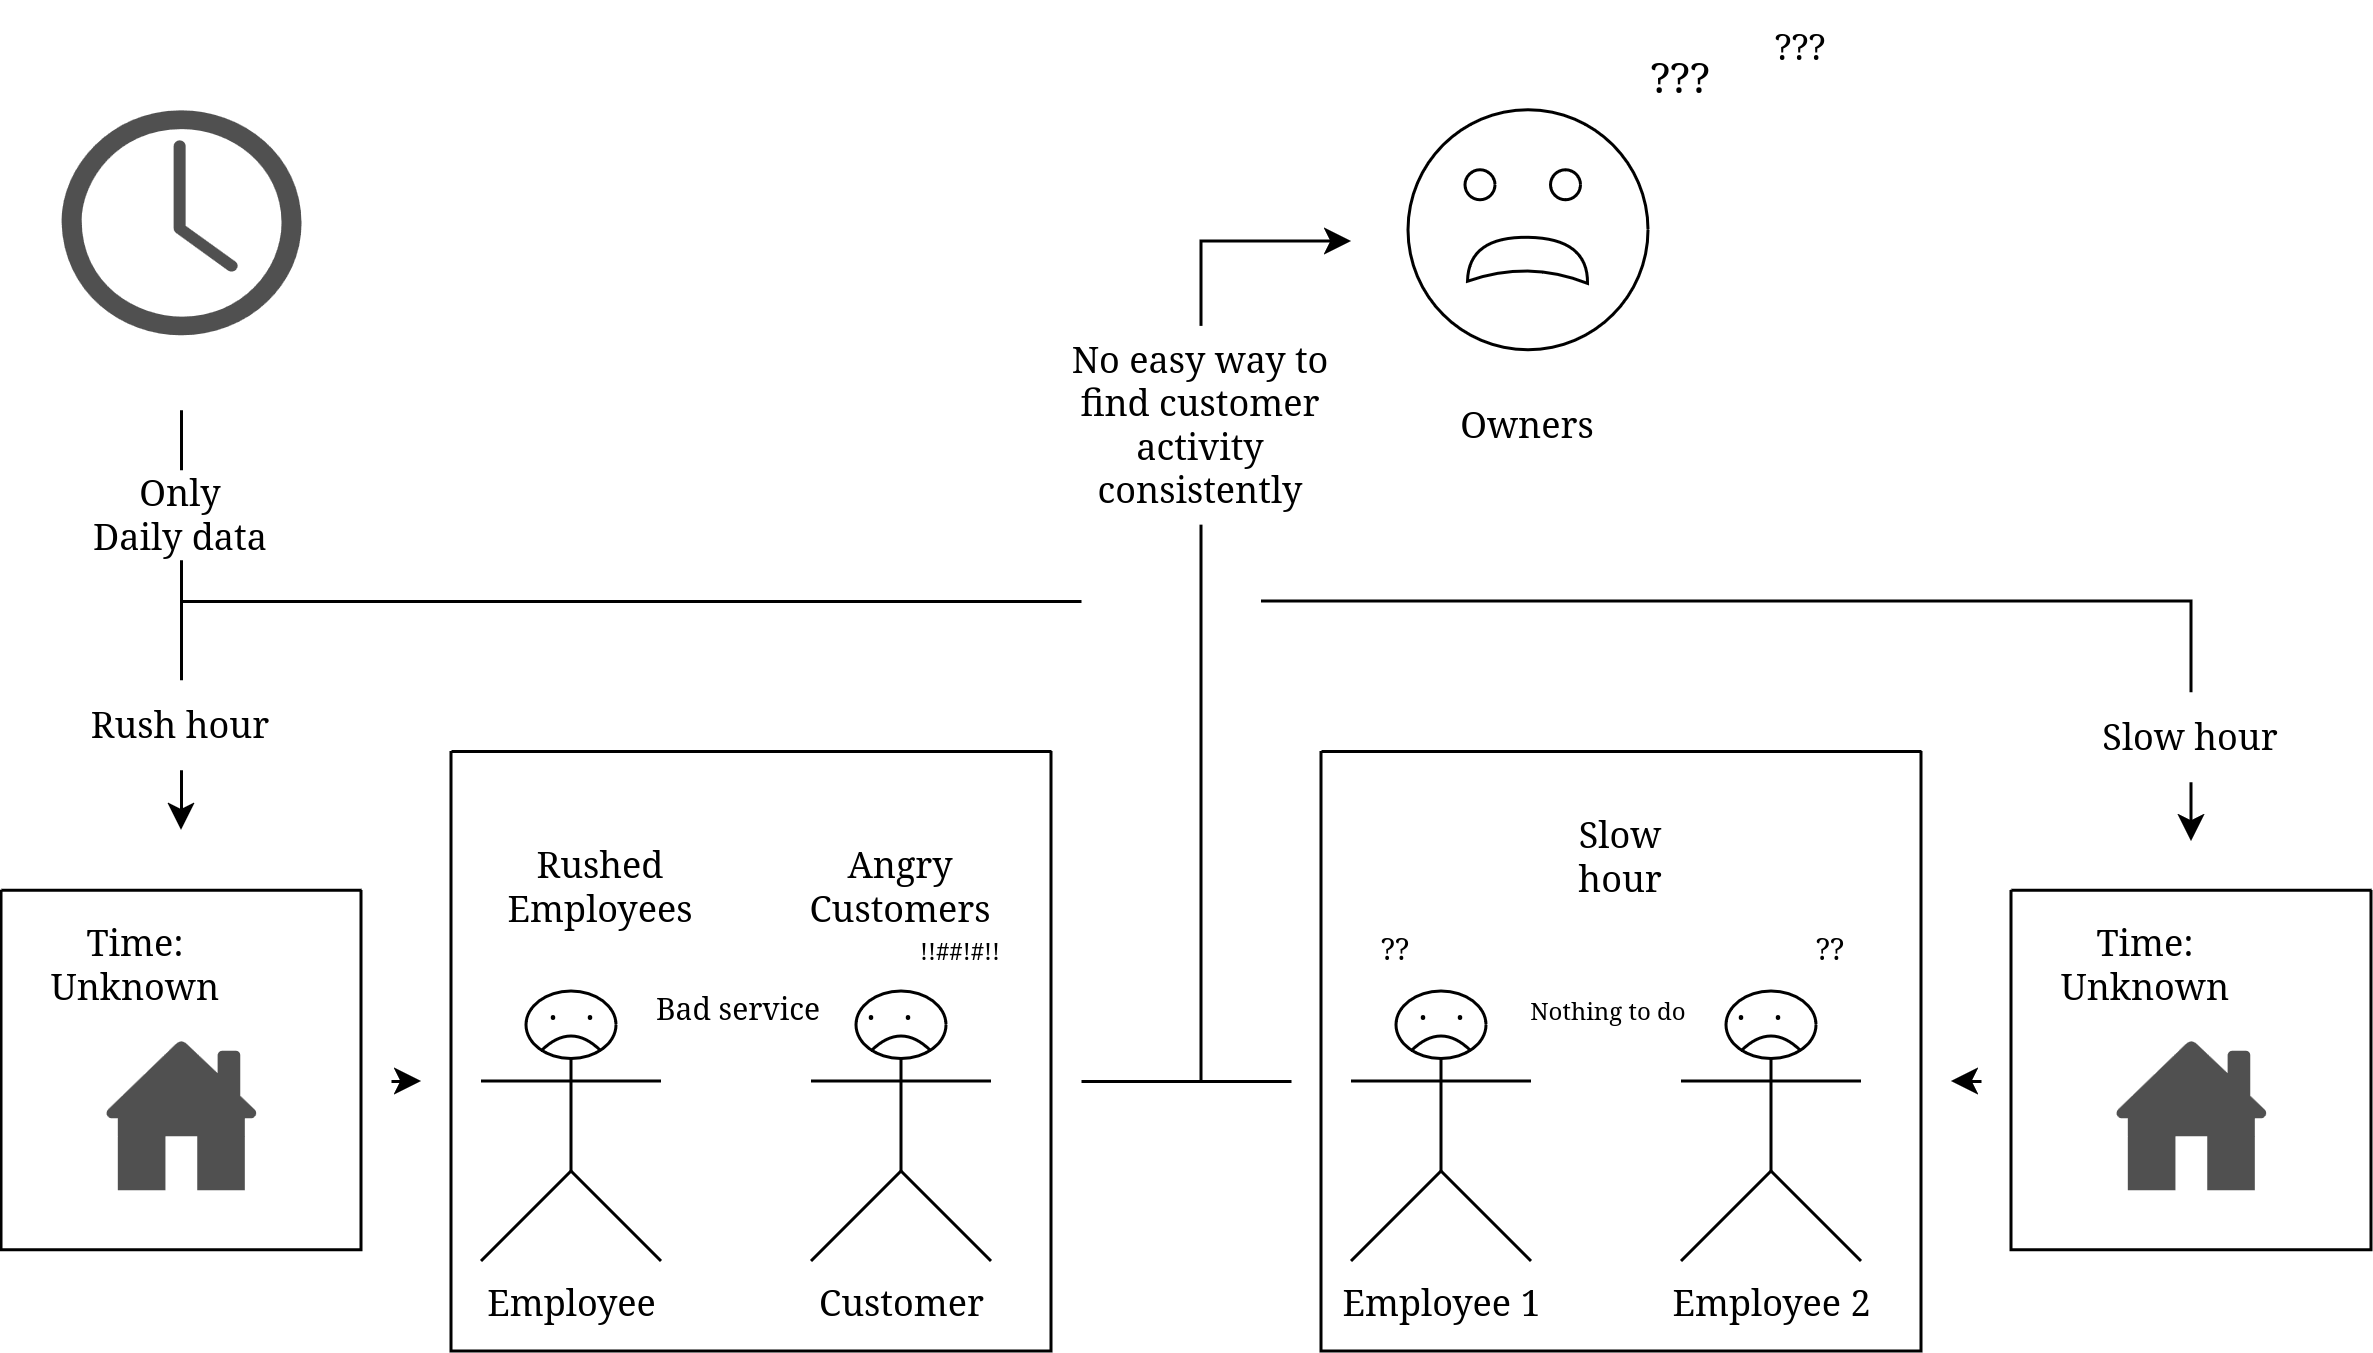
\includegraphics[scale=0.4]{rich_pictures_scheduling}
    \caption{Rich picture of the scheduling problem Nova café has.}\label{fig:pda-scheduling-problem}
\end{figure}
% textidote: ignore end
The figure depicts the likely outcomes of Nova not having hourly data about their customer activity,
which can likely end in bad customer service or the employee's not having enough work for multiple people.

The other issue that the authors will focus on solving for Nova is their food management difficulties.
Without detailed data on when specific items are sold, and in what quantity, it is challenging to plan
for when and how much they should make of their food products.
This can result in a large quantity of food having to be thrown out.
The inverse could also happen, which would be Nova selling out on popular products which stops them
from servicing customers.
This problem is visualized in~\ref{fig:pda-waste-problem}.

% textidote: ignore begin
\begin{figure}[!h]
    \centering
    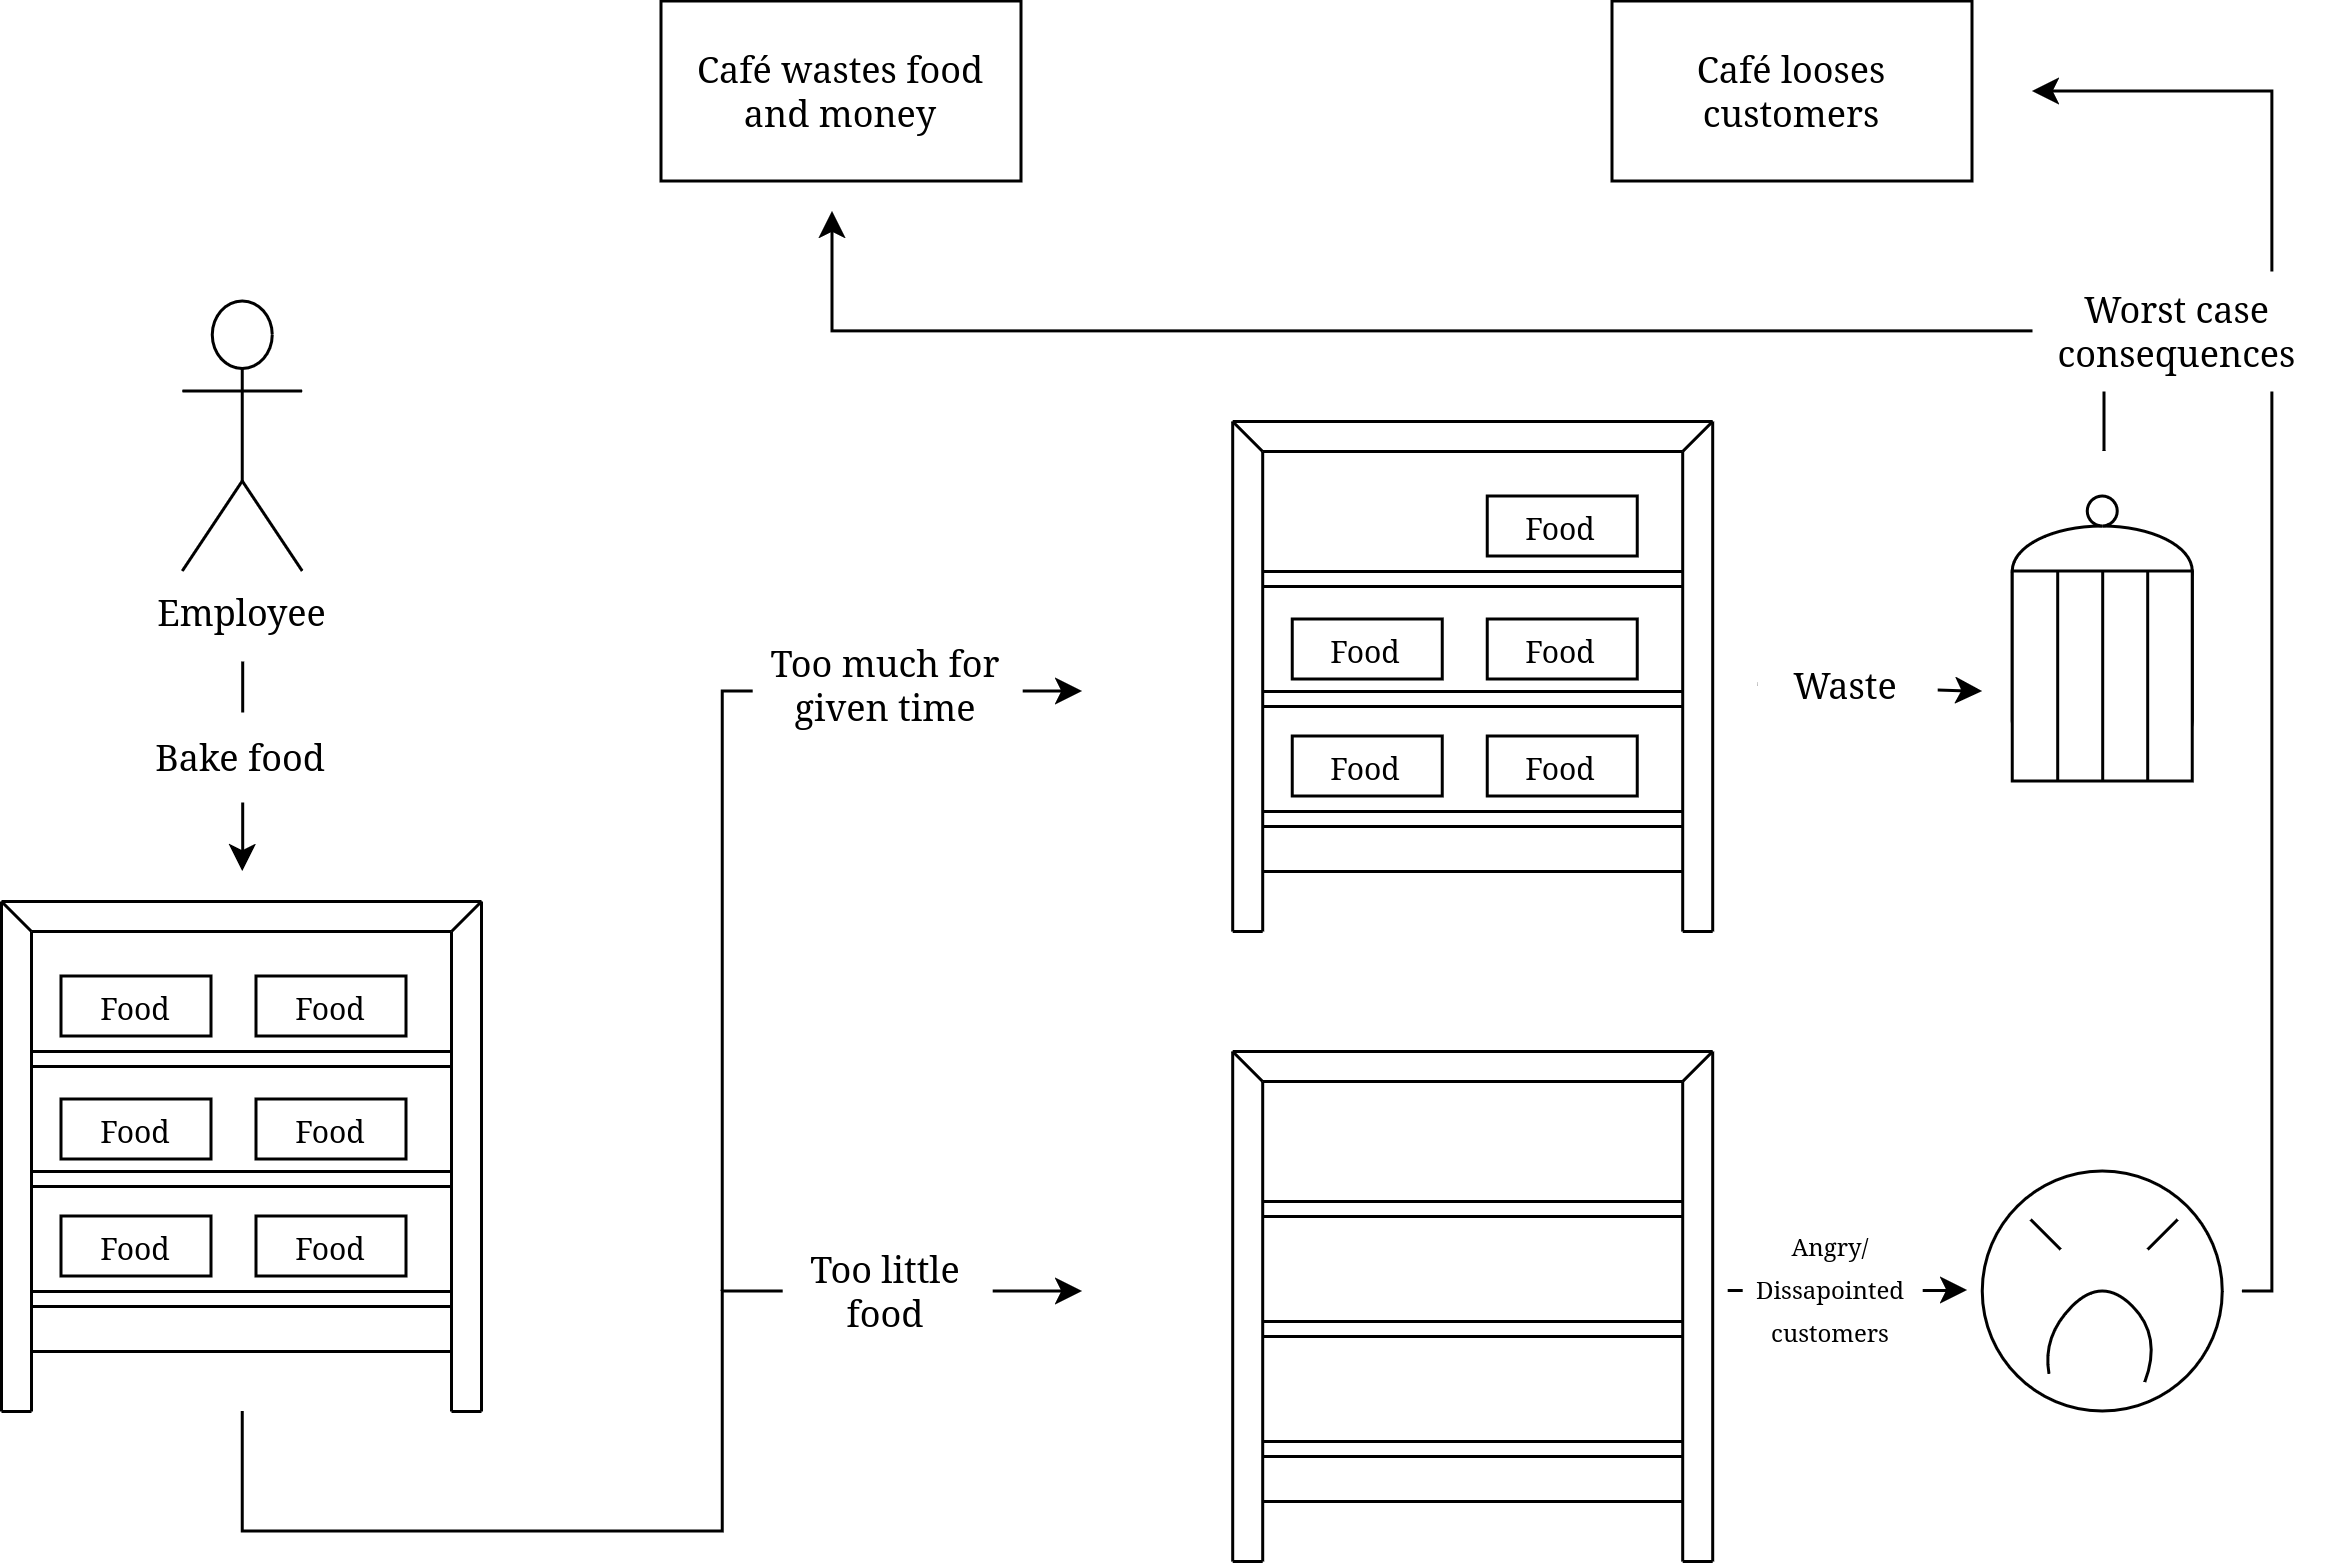
\includegraphics[scale=0.4]{rich_pictures_waste}
    \caption{Rich picture of the food waste problem Nova café has.}\label{fig:pda-waste-problem}
\end{figure}
% textidote: ignore end

\section{Problem statement}\label{sec:problem-statement}

When meeting the owners of the Caf\'e, they established that they wanted to have a system that could provide them with
an overview of their sales, so they could make better decisions based on their data.
The data provided by the system would help optimize staff shifts, ensuring that the right number of employees are
scheduled for the right time of day.

Additionally, the caf\'e sells baked goods that need to be prepared in advance.
The system should enable the owners to analyze the sales data provided to see the customer traffic from previous weeks,
ensuring they can prepare the right amount of baked goods for the upcoming days.

With one of the owners not being very tech-savvy, we would need to make sure that the system is easy to use and
understand, so it is critical that we focus on the UX of the system.

This presents us with the following problem statement:
\begin{tcolorbox}[title=Problem statement]
    How can we design an application that provides the caf\'e owners with a comprehensive overview of their sales and
    facilitates better decision-making based on the available data, while ensuring that the system is intuitive and
    accessible for all users?
    %textidote: ignore begin
\end{tcolorbox}
%textidote: ignore end

\subsection{Cultivating New Ideas}\label{subsec:cultivating-new-ideas}

During the initial consultations with the client NOVA Kaffe~\&~Vinbar, the group gained insight into the problem as seen
from the client's perspective.
For the next stage of the process, the group set on to try to gain a deeper understanding of the situation by
understanding existing solutions and brainstorming new ideas.

Whenever a new system is to be designed, it is crucial both to be able to objectively listen to the client and
understand the issue from their perspective.
Likewise, it is also crucial to understand whether any old, existing ideas have already solved the problem, since such
ideas could potentially be reused in the given situation.
Furthermore, new ideas need to be cultivated and evaluated in comparison to any existing solutions or ideas.
During this stage of the process, it is of vital importance to continuously brainstorm and evaluate ideas in
collaboration with the client, since, without such a collaboration, any prospective ideas might be too general or
abstract~\cite[32]{mathiassen2018}.

Therefore, the group conducted additional meetings with the client, where possible solutions were discussed.
One of the questions that the group asked the owners of NOVA was whether they were familiar with the Google Analytics
suite or Microsoft Power BI\@.
Both those pieces of software are extremely well-established in the industry and widely used, and can be categorized as
``old ideas'' that serve as \textit{exemplars}~\cite[33]{mathiassen2018} and form a potential solution for the problem.
Interestingly, the owners answered that they were familiar with the named software, but thought of it as either being
too complex to use, as in the case of Microsoft Power BI, or too general as Google Analytics.
Additionally, they expressed that neither of them had the necessary knowledge of data analysis or time to take care of
the prerequisite setup to be able to leverage the power of professional analysis software.
Rather, they hoped that a custom piece of software could be made with simplicity, accessibility and user experience in
mind — tailored to their needs, so to speak.

Now that the usage of existing solutions was eliminated, at least directly using them, one of the next questions was
whether the client already had some preconception of what such a custom piece of software could look like.
The client answered that they use an Apple iPad for all the daily operations of the café such as ordering inventory,
receiving payments through the~\acrfull{epos} system, managing staff, etc., and that they would love to be able to use
the custom software on the iPad.
Another requirement was that the software would present the business data through easy-to-understand data visualizations
that don't require knowledge of data analysis concepts.
The latter requirement was of special importance, since it also became clear that the software would have to be used by
all café staff, including young baristas, so accessibility once again appeared as a determining factor in the
discussions.

Continuing on the topic of preconceived ideas, the owners of NOVA told the group that they were thinking that an iPad
application would be the perfect software solution.
The reasoning behind this idea goes back to the fact that all the café's operations happen on the iPad anyway, so simply
having an additional app would be the most efficient scenario.
Now, the group pointed out a couple of obstacles with this approach: Namely, creating a one-off custom tablet
application is unsustainable, since it requires permission from the Apple App Store to be able to deploy it on the
café's iPad.
Such a permission would come with a fee and additional legal requirements, which the client didn't consider when first
discussing this idea internally before the meeting with the group.
So the group proposed an alternative: The application could easily run in the iPad's web browser, as a web application.
The owners of NOVA saw this proposal as a good balance between using the existing iPad infrastructure and ordering a
software solution that is economical, realistic and maintainable.

Next, the question of where the data to be analyzed would come from, and how it would be imported into the system
came up.
The primary source of all data, as the client explained, would be the business's~\acrshort{epos} system.
But the client also pointed out that a startup built the~\acrshort{epos}, which, due to its simple and new design,
lacked data exchange methods such as a public API, or similar.
The~\acrshort{epos} features data export in the form of CSV files, and, as the client explained, a requirement for any
future system would be that it can import those files easily and directly from the user interface.
Furthermore, because the data exported through CSV files from the~\acrshort{epos}, e.g., includes product IDs but no
product names, the data should be editable through the system's user interface.
This would facilitate that attributes such as product names can be added and mapped to file-imported product IDs.

And finally, since the two owners of the café were the sole administrators but not only employees of the business, an
additional requirement was placed that system admins should be able to add more users to the system, e.g., baristas.
This would enable the baristas to access the user interface using their own accounts, rather than relying on a primary
account, or creating an unauthenticated system.
Those users should have admin-editable and -removable accounts, so that the owners could administer the system according
to the current employees.

To conclude, the following requirements were deducted from the client meetings:
\begin{itemize}
    \item Easy-to-understand user interface.
    \item Data analyzed through visualizations.
    \item Target device and technology: iPad browser.
    \item Data imported into the system via a file.
    \item Data can be edited.
    \item Only owners (admins) can add, remove or edit other users.
\end{itemize}

\section{System Definition}\label{sec:system-definition}

The system definition, as per definition, is
\textcquote[23]{mathiassen2018}{[a] concise description of a computerized system expressed in natural language.}
Such a definition serves as the basis of any further procedures, due to it giving a specific perspective on the problem
at hand.
After consultations with the client, and the process of gaining deep, objective insight into the issues through the
consideration of different ideas, all the involved parties agreed upon one specific perspective.
The system definition that can be found down below attempts to reflect this perspective in a manner that can be
understood by everyone involved.
Furthermore, the definition also involves the interpretation of the system as stated through the statement earlier in
Section~\ref{sec:problem-statement}.

% textidote: ignore begin
\begin{figure}
    \centering
    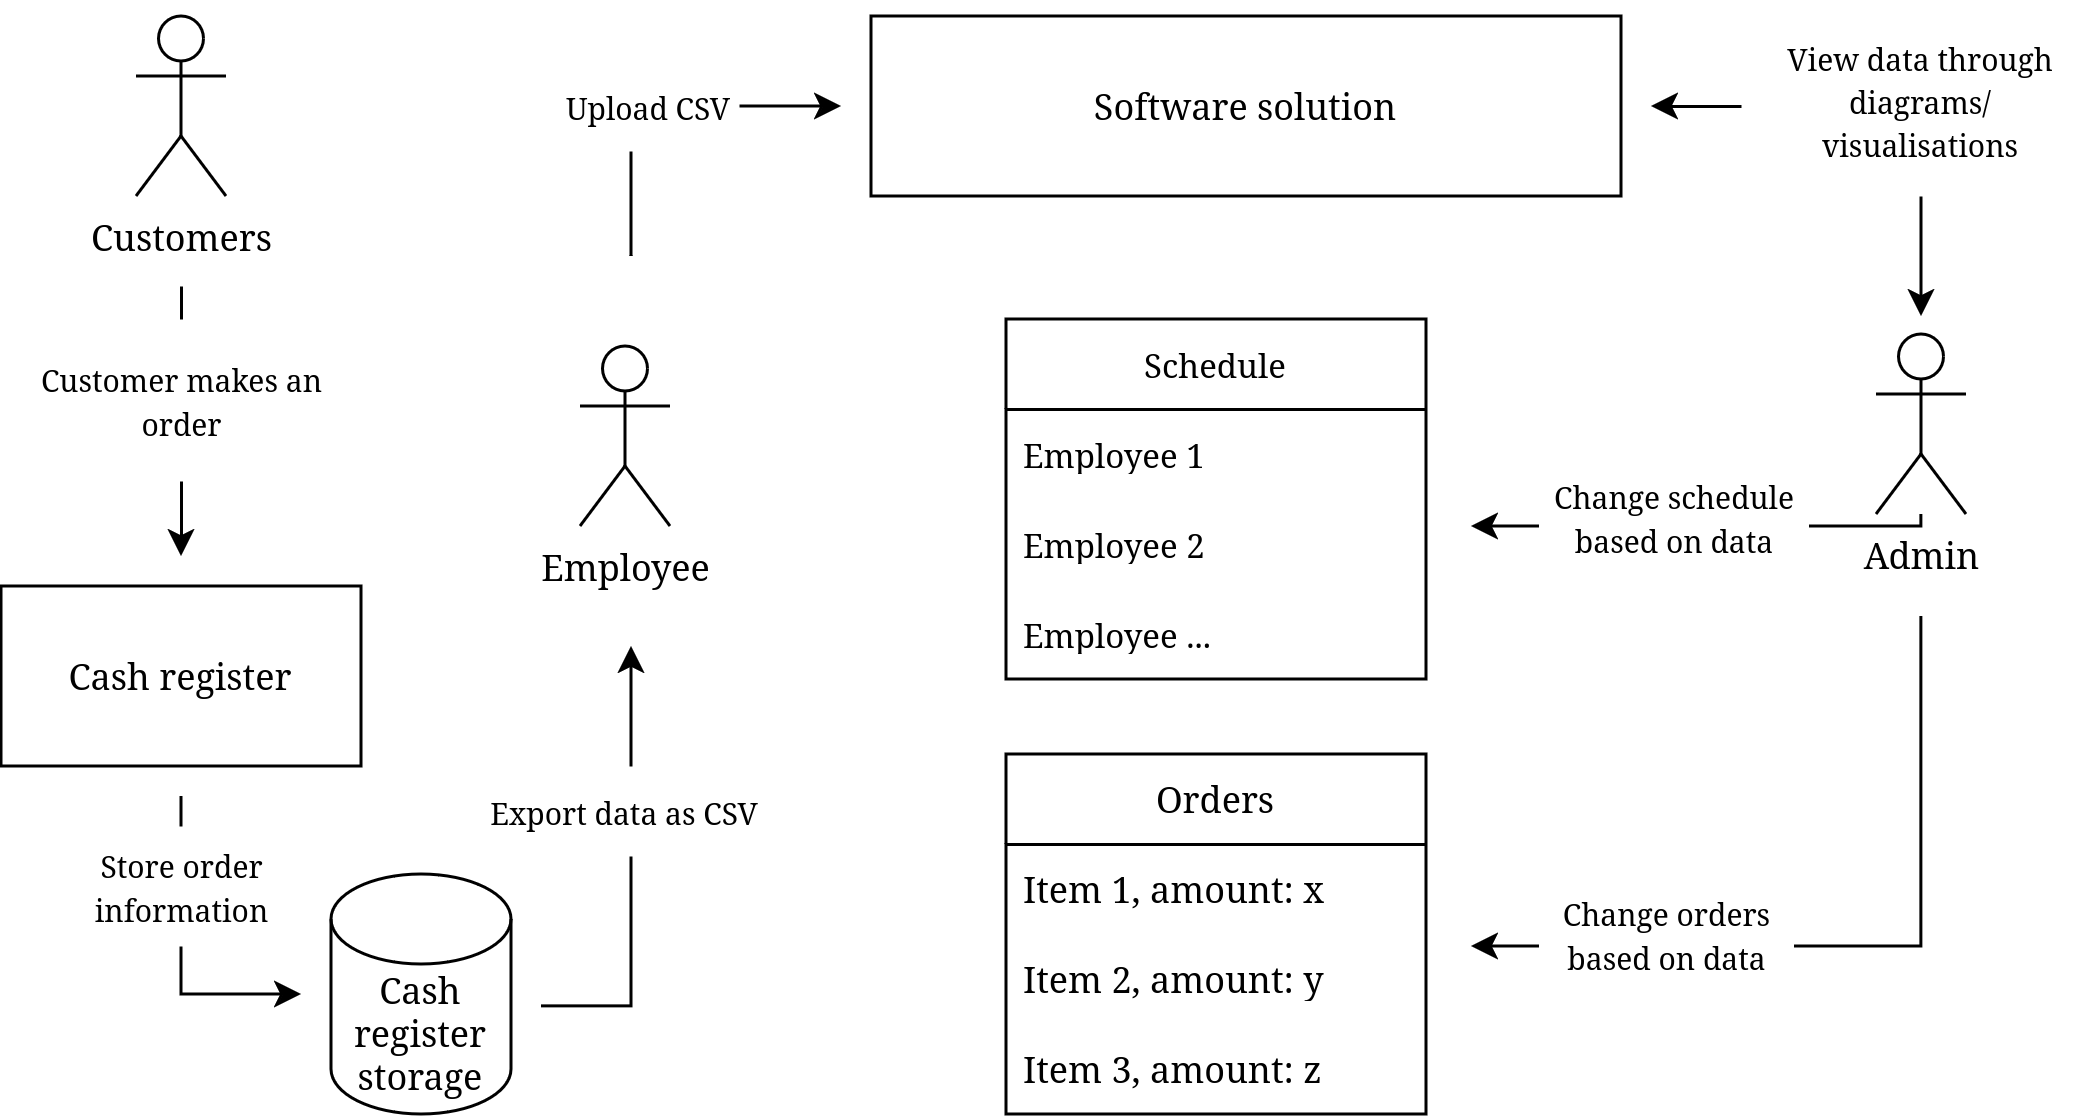
\includegraphics[scale=0.65]{rich_pictures_solution}
    \caption{A rich picture visualizing the proposed solution}\label{fig:pda-solution}
\end{figure}
% textidote: ignore end

Because system definitions also should reflect specific limitations~\cite[38]{mathiassen2018}, the group decided to
limit the system in terms of a specific user experience, target group, and system objective, rather than creating a
generalized system that also covers the client's needs.

Taking into consideration all the alternatives that were weighed, the following system definition was coined:
\begin{tcolorbox}[title=System definition]
    The digital system should enable NOVA Kaffe~\&~Vinbar to gain insight into their business, with emphasis on an
    easy-to-understand, graphical user interface.
    The user interface should, in particular, provide business insights through data visualizations.

    The system should serve the primary purpose of being an administrative tool, i.e., to improve the planning,
    purchasing, handling and distribution of human and business resources.
    For reasons of simplicity, accessibility and practicality, and taking into account that the primary users will
    access the system on a tablet device, the system should have a tablet-first web browser user interface.
    Management of users and the editing of data should be enabled for the owners, i.e., administrators of the system.

    Since the only possible integration of the proposed system with the outside world will be through file-based import
    of data, the system should facilitate such data imports in a user-friendly manner.

    Finally, the system should provide a simple enough user experience, enabling all employees at NOVA Kaffe~\&~Vinbar,
    regardless of their background knowledge, to make use of it.
\end{tcolorbox}

See depiction in~\ref{fig:pda-solution}.

% textidote: ignore begin
\section{FACTOR Criterion}\label{sec:factor-criterion}
% textidote: ignore end

The FACTOR criterion is a more detailed breakdown of the system definition~\ref{sec:system-definition}.
It is divided into six categories, each representing a different aspect of the system.

\begin{tabular}{ m{2.5cm} m{10cm} }
    \toprule
    \textbf{Category} & \textbf{Description} \\
    \midrule
    Functionality & The system should take the café's sales history as a comma-separated input data, and visualize it to
    help the user interpret the data and predict future sales. \\
    \midrule
    Application domain & The system will be used by the café's workers and managers, with the goal of getting an
    overview of the café's performance, and support them with food preparation and employee management. \\
    \midrule
    Conditions & The system will be developed by a group of students from AAU for use in NOVA, with the goal of solving
    their problem definition.
    As the system will be used by café workers, it must be user-friendly. \\
    \midrule
    Technology & The system will be deployed on a cloud server, which can be accessed through a normal web browser.
    It will primarily be accessed through the cash register, which is a tablet in this case, so the design must be
    mobile first. \\
    \midrule
    Objects & A list of objects can be found in the Section~\ref{sec:classes-objects-and-structure} \\
    \midrule
    Responsibility & The app must help users in decision-making when it comes to preparing for the day.
    This includes an efficient management of employees, insuring that the busiest hours have enough employees, and
    that enough food is prepared for the day. \\
    \bottomrule
\end{tabular}

\subsection{Software Requirements Specification}\label{subsec:software-requirements-specification}

For further clarification and alignment of features to prioritize the MoSCoW model is employed~\cite{hudaib2018}.
Herein an overview of the requirements for the software is covered.
\textbf{``Must-haves''} (Mo) include features that must be included in the software for it to be functional.
\textbf{``Should-haves''} (S) include features that are desired and possible to implement, but are not prioritized as
highly as must-haves due to time limitations.
\textbf{``Could-haves''} (Co) include features that are possible and valuable to implement but are not the main
focus of the report.
\textbf{``Won't-haves''} (W) include features that are out of scope and won't be implemented.

Furthermore, the requirements are split into two different tables, functional- and non-functional requirements as seen
in Table~\ref{tab:functional-requirements-specification} and Table~\ref{tab:non-functional-requirements-specification}
respectively.
Functional requirements describe what actions the system must be capable of performing.
Non-functional requirements, however, describe how the system must perform~\cite{benyon2019}.
This is done among other reasons to distinguish between functionality and quality attributes.
By having these separated into different tables, it is easier to plan design decisions and maintain a clear overview.

\begin{table}[H]
    \begin{tabularx}{\textwidth}{ l X X }
        \toprule
        \textbf{Functional requirement}
        & \textbf{MoSCoW annotation}
        & \textbf{Motivation}
        \\ \midrule
        Upload a~.csv-file
        & Mo
        & {\ul{\ref{subsec:cultivating-new-ideas}}}
        \\ \midrule
        Create a user
        & Mo
        & {\ul{\ref{subsubsec:classes-and-objects}}}
        \\ \midrule
        Delete a user
        & Mo
        & {\ul{\ref{subsubsec:classes-and-objects}}}
        \\ \midrule
        Create an order
        & Mo
        & {\ul{\ref{subsubsec:classes-and-objects}}}
        \\ \midrule
        Get a list of all orders with a particular product ID
        & Mo
        & {\ul{\ref{subsec:event-table}}}
        \\ \midrule
        Get a list of all orders on a particular date
        & Mo
        & {\ul{\ref{subsec:event-table}}}
        \\ \midrule
        Get a list of all customers
        & Mo
        & {\ul{\ref{subsec:event-table}}}
        \\ \midrule
        Delete an order
        & S
        & {\ul{\ref{subsubsec:classes-and-objects}}}
        \\ \midrule
        Update a user
        & S
        & {\ul{\ref{subsubsec:classes-and-objects}}}
        \\ \midrule
        Update an order
        & S
        & {\ul{\ref{subsubsec:classes-and-objects}}}
        \\ \midrule
        Export of data to an external file (e.g.\ CSV, JSON, etc.)
        & W
        & {\ul{\ref{subsec:factor-criterion}}}
        \\ \bottomrule
    \end{tabularx}
    \caption{MoSCoW model of the functional requirements specification.
    The \textit{Functional requirement} column describes the listed requirements for the software.
    The \textit{MoSCoW annotation} column covers the category to which the requirements belong.
    The \textit{Motivation} column encompasses where in the report the motivation for the requirements is located.
    }\label{tab:functional-requirements-specification}
\end{table}

\begin{table}[H]
    \begin{tabularx}{\textwidth}{ l X X }
        \toprule
        \textbf{Non-functional requirement}
        & \textbf{MoSCoW annotation}
        & \textbf{Motivation}
        \\ \midrule
        Data visualizations (graphs and charts)
        & Mo
        & {\ul{\ref{subsec:cultivating-new-ideas}}}
        \\ \midrule
        Usability in a tablet browser
        & Mo
        & {\ul{\ref{subsec:cultivating-new-ideas}}}
        \\ \midrule
        Data processing (raw data filtering and validation)
        & Mo
        & {\ul{\ref{subsec:system-definition}}}
        \\ \midrule
        A database
        & Mo
        & {\ul{\ref{subsec:system-definition}}}
        \\ \midrule
        The ability to handle a small number of concurrent users
        & Mo
        & {\ul{\ref{subsec:system-definition}}}
        \\ \midrule
        An intuitive and simplistic front-end design
        & S
        & {\ul{\ref{subsec:cultivating-new-ideas}}}
        \\ \midrule
        Mapping product ID to custom product name
        & S
        & {\ul{\ref{subsec:cultivating-new-ideas}}}
        \\ \midrule
        A well-structured codebase
        & S
        & {\ul{\ref{subsec:system-definition}}}
        \\ \midrule
        A fast and efficient frontend framework
        & S
        & {\ul{\ref{subsec:system-definition}}}
        \\ \midrule
        A robust backend framework
        & S
        & {\ul{\ref{subsec:system-definition}}}
        \\ \midrule
        Authentication via login
        & S
        & {\ul{\ref{subsec:system-definition}}}
        \\ \midrule
        Authorization of users
        & S
        & {\ul{\ref{subsec:system-definition}}}
        \\ \midrule
        Machine learning capabilities
        & Co
        & {\ul{\ref{subsec:system-definition}}}
        \\ \midrule
        A low response time
        & Co
        & {\ul{\ref{subsec:system-definition}}}
        \\ \midrule
        User-interactive data visualizations
        & W
        & {\ul{\ref{subsec:system-definition}}}
        \\ \midrule
        Other security measures (encryption)
        & W
        & {\ul{\ref{subsec:system-definition}}}
        \\ \midrule
        Scalability
        & W
        & {\ul{\ref{subsec:system-definition}}}
        \\ \midrule
        UI related semantic settings (color, language)
        & W
        & {\ul{\ref{subsec:system-definition}}}
        \\ \bottomrule
    \end{tabularx}
    \caption{MoSCoW model of the non-functional requirements specification.
    The \textit{Non-functional requirement} column describes the listed requirements for the software.
    The \textit{MoSCoW annotation} column covers the category to which the requirements belong.
    The \textit{Motivation} column encompasses where in the report the motivation for the requirements is located.
    }\label{tab:non-functional-requirements-specification}
\end{table}

